\chapter{Surface current on the waveguide walls}
In this chapter, we shall establish that the fields we got for rectangular waveguide if we take a limiting case that the fields must represent the ones we got for parallel plane waveguide. Now we do the work of showing that the field we got for a rectangular waveguide can represent the field we got for a parallel plane waveguide in the limiting case when one of the dimensions of the rectangular waveguide becomes infinity. We ask the question what happens to the mode which was $TM_0$ which becomes the TEM mode in the parallel plane waveguide? What happened to that mode in a rectangular waveguide? Does this mode now exists inside the rectangular waveguide or it exists only inside a parallel plane waveguide?
\begin{figure}[h]
\centering
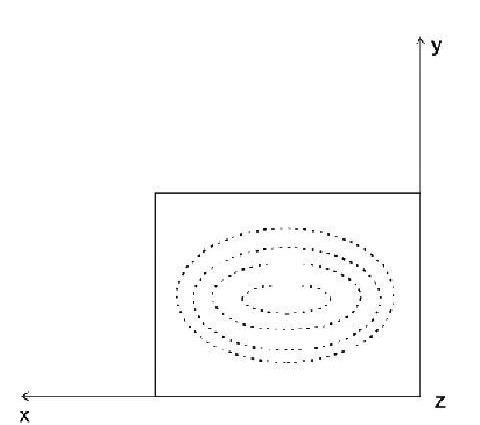
\includegraphics[width=0.6\linewidth]{./graphics/group4001}
\caption{}
\end{figure}
 So we consider the question does a TEM exist inside a rectangular waveguide? Using the rectangular wavelength, we could find out that the electric and magnetic fields are both perpendicular to the direction of propagation. That means they must lie in the XY plane below. That means they must perform a closed loop in the plane. Then there has to be CURRENT enclosed by the magnetic field lines, then and only then can the magnetic field lines survive. Hence there would either be a CONDUCTION or DISPLACEMENT current that will guarantee the survival of the magnetic field lines since we do not have any conducting medium inside the waveguide, it is completely hollow, with pure dielectric inside, and there is no possibility of conduction current enclosed by the magnetic field lines. Hence conduction current is zero inside the rectangular waveguide, so magnetic field lines can only be sustained by the fact that we have a displacement current, and it must be following in the z-direction. This displacement current will also require an electric field going in the z direction which will already say is not there for TEM mode. We said the electric field only lies on the transverse plane for TEM mode. It does not have a component perpendicular to the plane of the paper.

If that is so, we cannot have the displacement current inside the waveguide that is in the z direction, so either we have a conduction current or displacement current going in the Z direction. So there is no current which is flowing perpendicular to the plane of the paper, and hence there is no current sustaining the magnetic field lines. As by amperes law, the magnetic field lines must enclose current. This means that these fields which are lying in the transverse plane cannot exist, as there are no currents to support the magnetic field lines. That means the TEM cannot exist inside a rectangular waveguide, so TEM mode DOES NOT EXIST IN a RECTANGULAR WAVEGUIDE.

Let us take a parallel plane waveguide as a limiting case of a rectangular waveguide. If we take the rectangular waveguide in mode is existing and make ${b=\infty}$, we get a structure mode of only side E and G left, and the wave is going to travel in the Z direction. So if the electrical field was on the plane of the paper and the wave is going to propagate in the Z direction, this would essentially correspond to the TE mode. So with sides, E and G left and an electric field on the plane of the paper in the Y direction, we would get a geometry which is the parallel plane geometry which gives the TE mode. We can understand better from the diagram shown below.
With an electric field in the Y direction as shown below,\\
${E_x = E_z = 0 \qquad E_y = - \dfrac{j\omega\mu a}{\pi} Csin(\dfrac{\pi x}{a})e^{-j\beta z}}$\\
$H_x = + \dfrac{j\beta a}{\pi} Csin(\dfrac{\pi x}{a})e^{-j\beta z}$\\
$H_y = 0\qquad H_z = Ccos(\dfrac{\pi x}{a})e^{-j\beta z}$ and magnetic field ${H_x}$ and ${H_z}$ for this case had.
\begin{figure}[h]
\centering
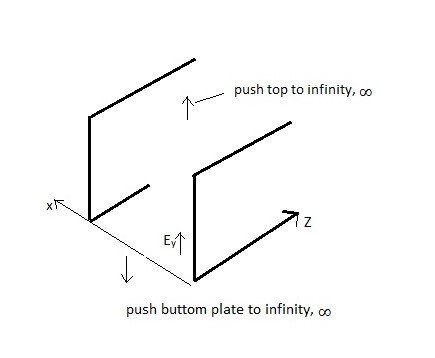
\includegraphics[width=.7\linewidth]{./graphics/page3}
\caption{}
\end{figure}
and all these fields were constant as a function of Y.Some thing we can get now with ${b=\infty}$ that is there are no boundary conditions to apply in the Y direction. The field is infinite, then ${E_y}$ is constant along Y direction. That is precisely the field we used to get a parallel plane waveguide. So in rectangular waveguide,we can take ${TE_{10}}$ mode and make b in infinity and since we do not have any dependence of E here on y,it means that the fields in the ${TE_{10}}$ case are essentially the same for a parallel plane waveguide. So the ${TE_1}$ mode of a parallel plane waveguide has essentially the same field as ${TE_{10}}$ mode of a rectangular waveguide, Now we have a Z magnetic field in the z-direction. So in the limiting case of the ${TE_{10}}$ mode,we can get the transverse electric mode lowest order transverse electric mode which is $TE_1$ mode and it will be exactly what we got for ${TE_{10}}$. Another mode we had was the TEM mode for which the electric field was not tangential to the boundaries,(i.e along x above)the magnetic field was tangential to the boundary (alone y direction)and we say that was the mode which was not dispersive and travels as if the conducting boundary are not existing and that was the mode which was the TEM mode. We had the diagram below that if we take a parallel plane waveguide, the electric and magnetic field is shown in the direction below. 

The wave travels without any variation of the electric and magnetic field as we saw earlier because neither H requires the boundary conditions to be satisfied which is tangential, so we can always have surface currents, nor the normal components of an electric field needs only boundary condition to be satisfied.We can always have the surface charge induced to compensate for the normal component of the electric field.So this mode which was the TEM mode was existing inside the parallel plane waveguide.
\begin{figure}[h]
\centering
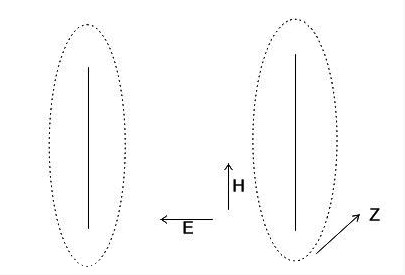
\includegraphics[width=.7\linewidth]{./graphics/page4}
\caption{}
\end{figure}
One can ask the question that if the figure above was the limiting case of the rectangular waveguide, how come this mode exist in the parallel plane waveguide,but when we take a rectangular this mode does not exist!We argue that since the magnetic field is in the Y direction and the plane is extended in the Y direction and this means the magnetic field lines essentially close at infinity and enclose the conductions shown by dotted lines.These conduting plane have a surface current flowing on them.In the case of rectangular waveguide were those boundaries are finite,the magnetic field closed on themselves and current is enclosed.That is why the TEM mode cannot exist in rectangular waveguides.But with a parallel plane structure,the magnetic field lines will close at infinity and will enclose the plane conductors as shown above and so the TEM mode can exist inside a parallel plane waveguides.This is the mode like we say in two conductor system like coaxial cables,this mode propagates.

So whenever we have a two conductor system,the lowest mode which will propagate will be TEM mode,however if we go to the rectangular waveguide,the lowest mode which will propagate will be ${TE_{10}}$ mode.The important conclusion to draw is that whenever we have a hollow structure,like a hollow pipe kind of waveguide,tyhe TEM mode cannot exist which is non dispersive.It is a special mode that is not supported by the rectangular waveguide. That is why we have all the problem of dispersion and so on,inside a rectangular waveguide. The parallel plane waveguide is still a structure which is infinite in extent,it cannot be realized in practise.It is good for understanding,but when we want to realize the structure in practise,it is the rectangular waveguide which can be realized practise,not the parallel plane waveguide,so whenever if we have a physical structure which is a rectangular waveguide,we always have a cut off frequency associated with that and we always have problem like dispersion and so on,associated with them.

With this understanding,let us try to see the current which gets excited on the walls of the waveguide,which actually support these fields inside the waveguide.So whether we take a parallel plane or rectangular waveguide,what is the mechanism by which these fields are supported inside the waveguide? what are the sources? The sources are nothing but surface charge and surface currents which lie on the inner surface of the waveguides.So as the wave travels even the surface charge keeps moving i.e accumulate at different locations as we see later and these charges and surface currents supports the electric and magnetic field inside the waveguide which is responsible for carrying power inside the waveguiding structure.So what we do now,is first we try to visualize the fields which would be inside the waveguide and then try to visualize how the currents are disturbing on the walls of the waveguide, so let us take the simplest case which is the TEM case for a parallel plane waveguide in the parallel plane waveguide shown for TEM mode,the electric field E is perpendicular to the plans.With\\
${E_y = Ce^{-j\beta z}}$ and ${H_x = \dfrac{C}{\eta}e^{-j\beta z}}$ We can visualize these fields.if we tried out how these fields are going to be a function of space and time in the structure.First we freeze time,remember all the qualities above are intrinsic function of time.So ${e^{j\omega t}}$ is implicit in all the terms\\
$E_y = Ce^{-j\beta z}e^{j\omega t}\qquad H_x = {\dfrac{C}{\eta}}e^{-j\beta z} e^{j\omega t}$
\begin{figure}[h]
\centering
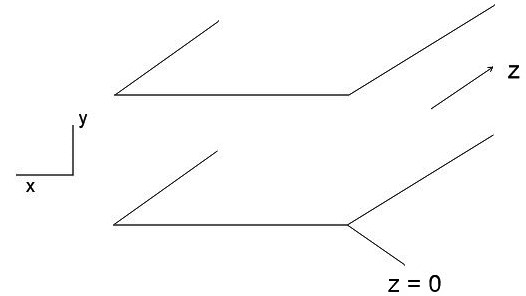
\includegraphics[width=.7\linewidth]{./graphics/page6}
\caption{}
\end{figure}

So these fields are varying as a function of space and time,so if we stand at a particular location in space, the field will vary as a function of time.if we freeze time or say at any instant of time,we look along the waveguide,we see a variation given as ${e^{-j\beta z}}$ so to visualize these fields in 3D, first we freeze time i.e make ${Wt}$ constant.At that instant,we want to see how the field are disturbed in space. Once we get those fields disturbing in space, then we essentially say that these field will be moving with a phase velocity for the mode. Then the electric field drift inside this waveguide with the phase velocity. So when we visualize these fields, essentially we try to visualize the spatial variation of the fields at some instant of time and without loosing generally,we can take the time t=0. If we take t=0, i.e freeze time,then the field visualization is simply the real part of ${H_y}$ and${H_x}$ which is \\
${Re\{Ce^{-j\beta z\}}\}}$ and ${Re\{\dfrac{C}{\eta}e^{-j\beta z}}\}$ That is ${Ccos\beta z}$ and ${\dfrac{C}{\eta}cos\beta z}$ If we consider points Z=0,with variation of ${\beta z}$
so the field varies as a cosine function in direction Z. It is constant in XY plane, so we see the cosine variation along the Z direction for these fields.The electric field is same at any Z(i.e XY plane)and in the Y direction.
\begin{figure}[h]
\centering
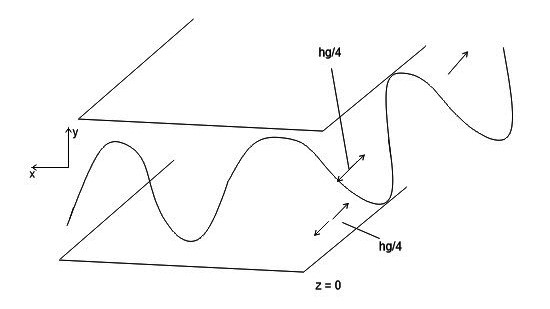
\includegraphics[width=.7\linewidth]{./graphics/group4002}
\caption{}
\end{figure}
\begin{figure}[h]
\centering
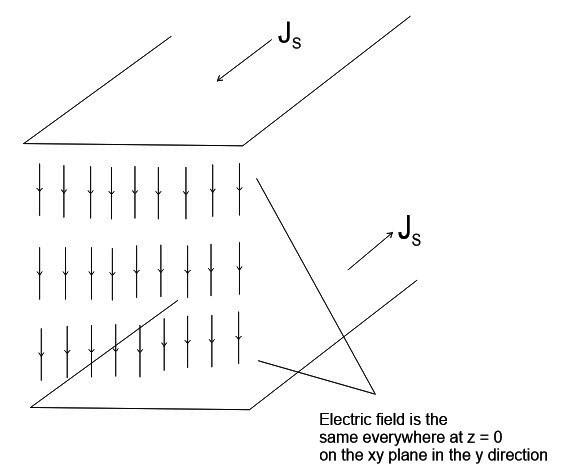
\includegraphics[width=.7\linewidth]{./graphics/page702}
\caption{}
\end{figure}
\begin{figure}[h]
\centering
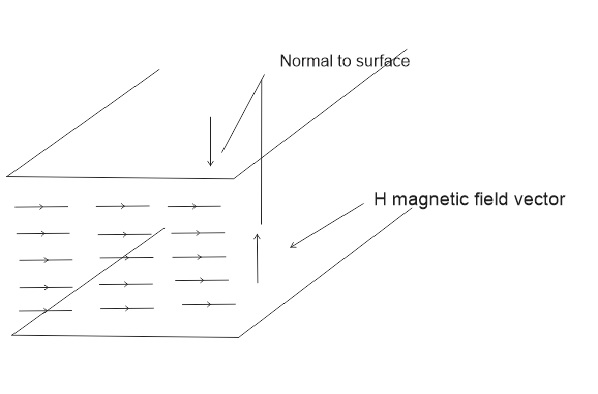
\includegraphics[width=.7\linewidth]{./graphics/page703}
\caption{}
\end{figure}

The magnetic field is same at Z(XY PLANE)and in the X direction.The E and H direction is maintained to show the direction of propagation by poynting theorem(a british physicist John Henry Poynting). So E start maximum will H maximum at Z=0 \quad${A\quad Z= \dfrac{hg}{4}}$they have reduced to zero. Beyond ${Z= \dfrac{hg}{4}}$,they change direction and start increasing till they go to another maximum at ${Z=\dfrac{hg}{2}}$ They again start decreasing from the direction of ${Z=\dfrac{hg}{2}}$ to ${Z=\dfrac{3hg}{4}}$where E and H are zero.Beyond ${Z=\dfrac{3hg}{4}}$,  they change direction once more and start increasing getting to Z=0 state at ${\lambda g}$.With little practice one can see how the electric and magnetic field varies inside the waveguide.Now we know that if that if the magnetic field pattern is as shown above,the current which is going to flow in the surface of the conductor is related to the magnetics fields i.e the tangential component of the magnetic fields.The ${\hat{n}\times\bar{H}}$.gives the surface currents on the conducting walls. Since we are considering here ideal conductors,essentially,calculating ${\hat{n}\times\bar{H}}$, that is the current which is truely confirm to the surface of this parallel plane waveguide. 

The normal to surface of H fields is shown. We choose the normal pointing inwards as that is the part that bounds the electromagnetic wave to be propagated.The normal opposite that would be the electromagnetic wave was propagated outside the conducting plane. So the unit vector of the wave plane is going upward in ${\hat{y}}$ direction for the upper plane in ${-\hat{y}}$ direction. Now we can calculate ${\hat{n}\times\bar{H}}$. The ${\hat{n}\times\bar{H}}$ will give the direction of surface current,which top plane, ${\hat{n}\times\bar{H}}$ is -Z direction as to say the surface current is coming out from top plane and going in the bottom plane.Hence ${J_s}$ direction shown on the top and bottom plane respectively.${J_s}$ will be having same variation as the variation of the magnetic field. Maximum at Z=0, and ${Z= \dfrac{hg}{4}}$.Maximum at ${Z=\dfrac{hg}{2}}$ but with direction reversed, zero at ${\dfrac{3hg}{4}}$ and maximum again at ${Z=hg}$

with same direction as with Z=0. So in a two conductor system, we get current flow in the direction in which the wave is propagating. ${J_s}$ in the +Z direction in the bottom at Z=0 and ${J_s}$ in -Z direction at the top for Z=0. If we have a two conductor system like the coaxial cable,we connect a voltage source,current goes inside the conductor and returns back through what is called a ground path.So we see that the current goes inside from one terminal and comes outside from the other terminal. So in that situation of the two conductor system, the direction of the current flow which we have for the TEM mode(keep in mind) is the same as the direction of wave propagation.So current is going from bottom plane and returning from top plane at Z=0.The question me ask is if the wave is propagating in the Z direction ,is it always true that current has to flow in the Z direction or direction of wave propagation? Then we got the answer which is wrong.That is since we always discuss the transverse electromagnetic mode.
\paragraph{}The fact that we are used to when we go to low frequency circuit,immediately we jump to the conclusion that yes since the wave is moving in the Z direction,the power is flowing in the Z direction,the current must flow in that direction.
\begin{figure}[h]
\centering
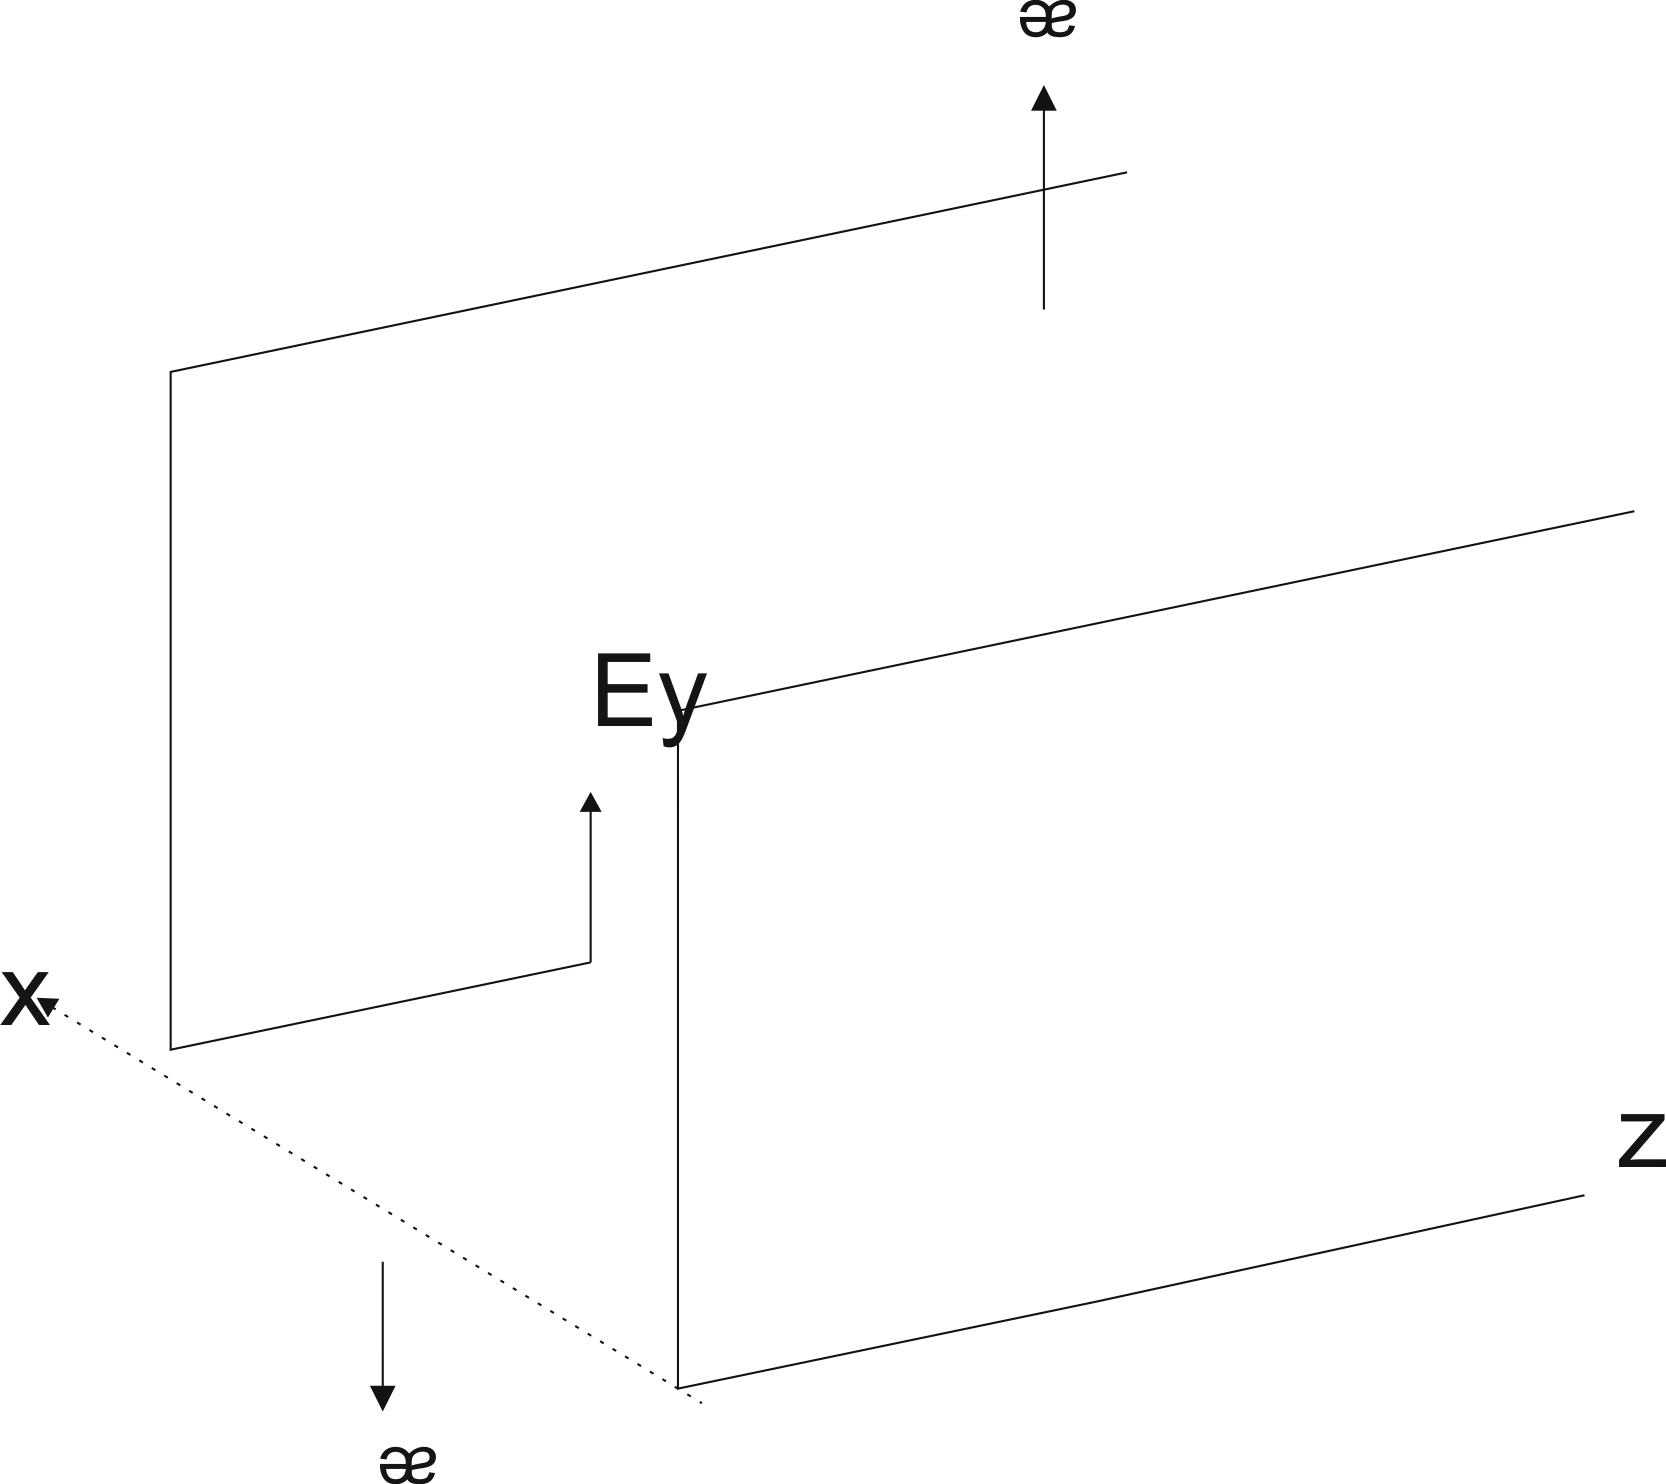
\includegraphics[width=.7\linewidth]{./graphics/WATSON4}
\caption{}
\end{figure}
\paragraph{}Let us look at the parallel plane waveguide,let us take a mode which is TE mode and let us see what will be the direction of current and field in the waveguide.As we saw ,the fields for the parallel plane waveguide is identical to the $TE_{10}$ mode for rectangular waveguide giving as\\
${E_x = E_z = H_y = 0}$\\
$E_y = -\dfrac{j\omega \mu a}{\pi}Csin(\dfrac{\pi x}{a})e^{-j\beta z}$\\
$H_x = -\dfrac{j\beta a}{\pi}Csin(\dfrac{\pi x}{a})e^{-j\beta z}$\\
$H_z = Ccos(\dfrac{\pi x}{a})e^{-j\beta z}$

So the electric field will be y oriented,it will have a variation which would be in the Z direction. With very in the Z direction with the value of ${\beta}$.To visualize ${E_y}$, lets take the real part of ${E_y}$ and look at its variation,and with respect to x,y and z. This will give us a 3 dimensional picture of the fields.\\
$E_y = \dfrac{-j\omega \mu a}{\pi}Csin(\dfrac{\pi x}{a})e^{
-j\beta z}\equiv e^{-j\dfrac{\pi}{2}}\dfrac{\omega \mu a}{\pi}Csin(\dfrac{\pi x}{a})e^{-j\beta z}$\\
${E_y = \dfrac{\omega \mu a}{\pi}Csin(\dfrac{\pi x}{a})e^{-j(\beta z + \dfrac{\pi}{2})
}}$\\
Real ${(E_y) = \dfrac{\omega \mu a}{a}Csin(\dfrac{\pi x}{a})cos(\beta z + \dfrac{\pi}{2})}$\\
${[cos(-(\beta z + \dfrac{\pi}{2}))=cos(\beta z + \frac{pi}{2})]}$\\
cosine is even function\\
${\dfrac{\omega \mu aC}{\pi}\equiv A}$, we have Real ${(E_y = Asin(\dfrac{\pi x}{a})cos(\beta z +\dfrac{\pi}{2})}$ ,
Real ${(E_y)= Asin(\dfrac{\pi x}{a})sin(\beta z)}$\\
${= Asin(\dfrac{\pi x}{a})sin(\dfrac{2\pi z}{hg})}$ we can do some thing for ${H_x}$\\
Real${(H_x)= Bsin(\dfrac{\pi x}{a})sin(\dfrac{2\pi z}{hg})}$\\
Real${(H_z)= Ccos(\dfrac{\pi x}{a})cos(\dfrac{2\pi z}{hg})}$\\
Real${(E_y)= Asin(\dfrac{Hx}{a})sin(\dfrac{2\pi z}{hg})}$
 These are the field which are in existence when time is fixed,say at t=0. At that instant, these three expressions gives the fields along the waveguides.\\
 As we can see in the Z direction,the field are all sinusoidal with a spatial period of ${hg}$. However ${Re\{H_x\}}$ and ${Re\{H_z\}}$ are in QUADRATURE. That is ${90^{o}}$ degree out of phase with each other. So when ${H_x}$ is maximum,${H_z}$ is zero.When ${H_z}$ is maximum,${H_x}$ is zero. So in space we have two components now, the ${H_x}$ and the ${H_z}$ components.${H_x}$ component has sine variation along Z,with Z=0, ${H_x}$ is zero at that location, but ${H_z}$ in Z direction is maximum at that location. If we go ${Z=\dfrac{hg}{4}}$, ${H_x}$ is maximum and ${H_x=0}$. Looking from the top, it will appear.
\begin{figure}[h]
\centering
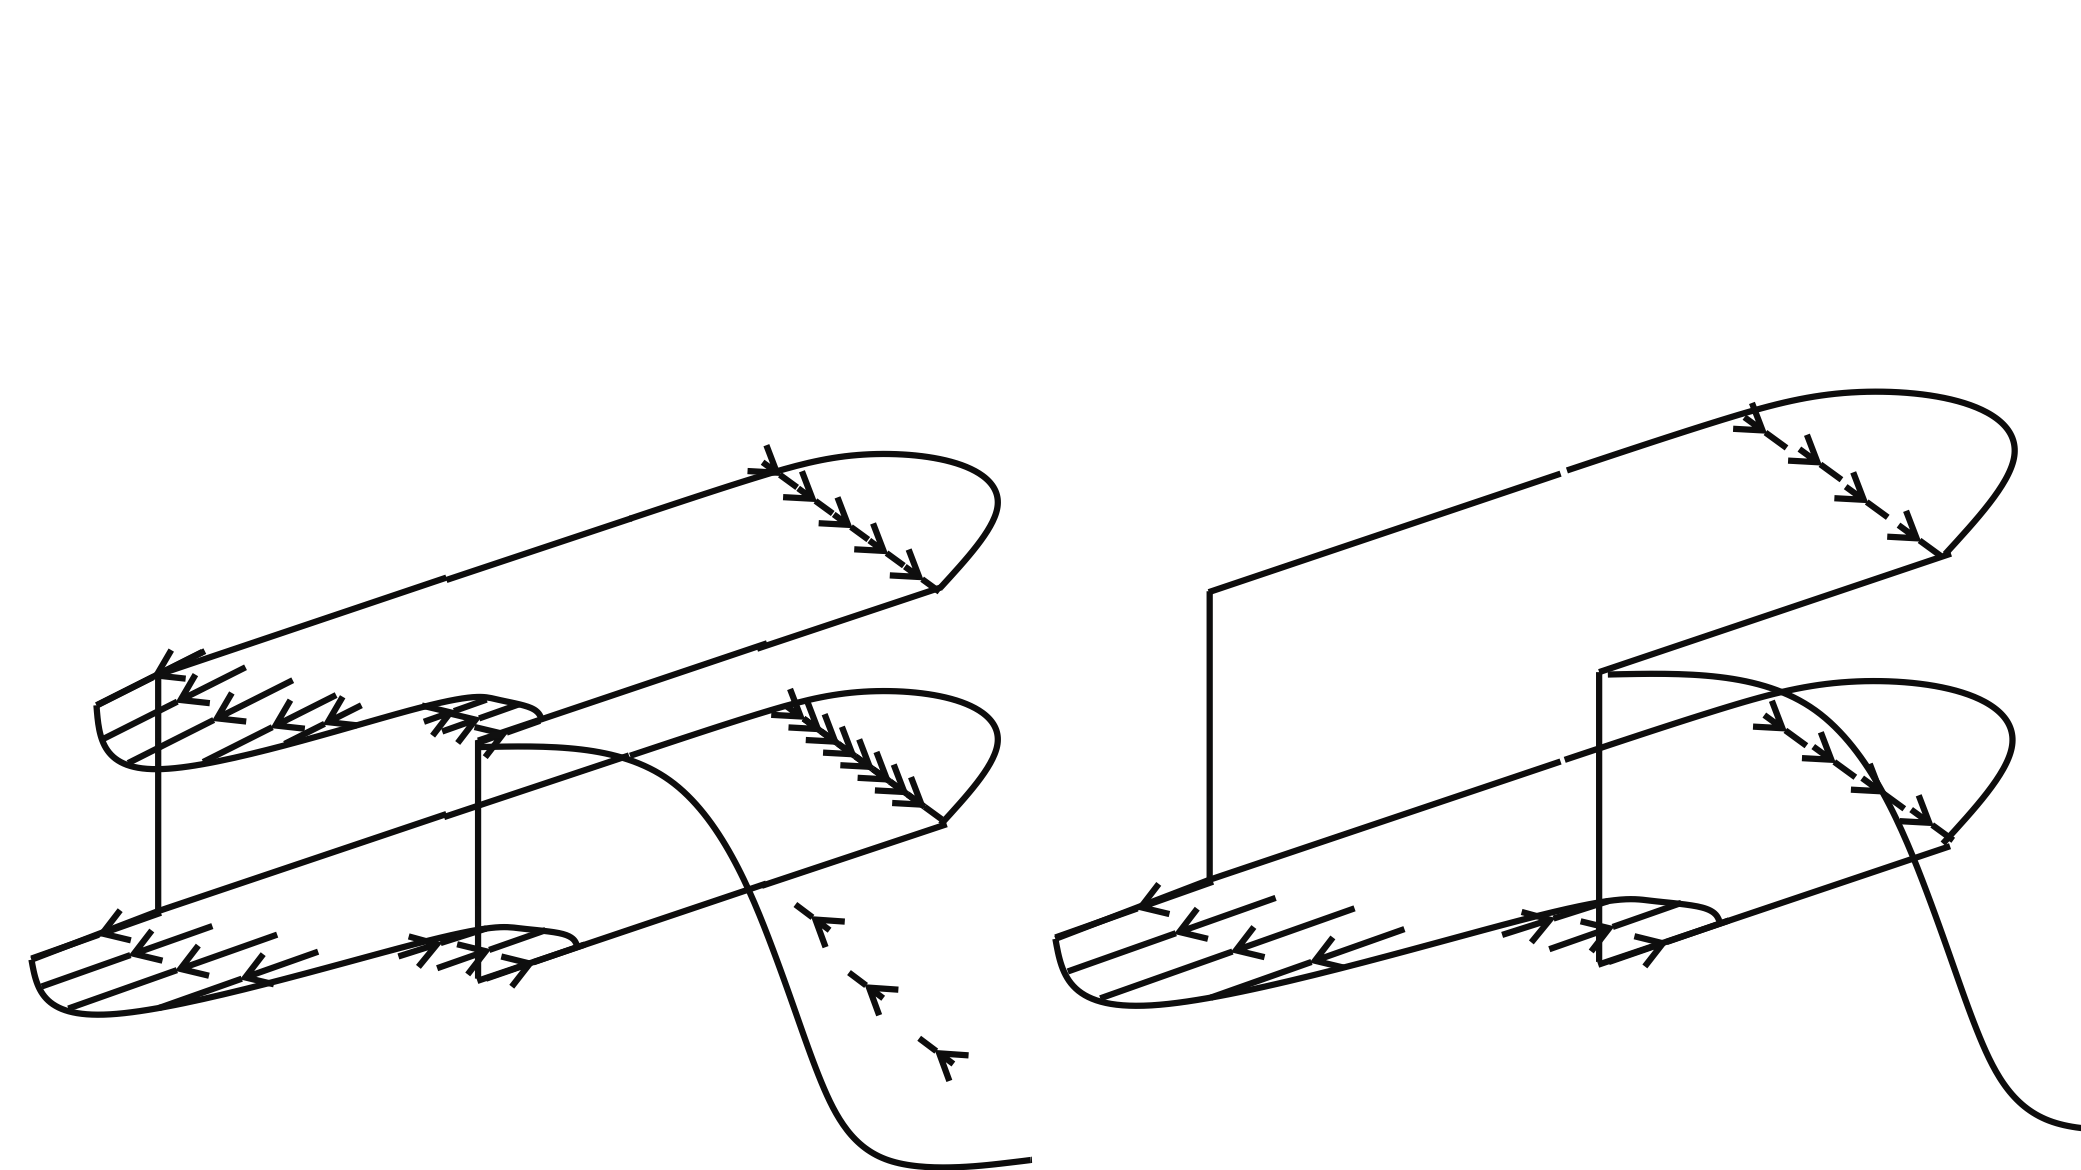
\includegraphics[width=1\linewidth]{./graphics/WATSON}
\caption{}
 \end{figure}
 From the top for this parallel plane waveguide,we see the magnetic fields below.Since the magnetic field close on themselves,it is only a matter of imagination.
 % \begin{figure}[h]
 %	\centering
 %	\includegraphics[scale=0.1]{""}
 %	\caption{}
% \end{figure}
to close the magnetic field loops as shown by the dotted lines ${\dfrac{hg}{4}}$ from here the direction with reverse to have the dotted line from $\dfrac{hg}{4}$  to $\dfrac{hg}{2}$ and so on.
 % \begin{figure}[h]
 %	\centering
 %	\includegraphics[scale=0.8]{""}
 %	\caption{}
 %\end{figure}

Hence we can complete this to get the field distribution below, for a waveguide going from ${-\infty}$ to ${+\infty}$.\\
So from the top in a parallel plane waveguide, the magnetic field lines look like rolled carpets which are scattered inside the structure. They are of infinite length perpendicular to the plane of the paper. This is how the magnetic field will be distributed.

However for the electric field, ${E_y= Asin(\dfrac{\pi x}{a})sin(\dfrac{2\pi z}{hg})}$ the electric field has variation in the Z direction since as ${H_x}$,but it is oriented in the y direction.So from top the electric field lines is perpendicular to the plane of the paper. The behave of ${E_y}$ and ${H_x}$ is identical. That means whenever ${H_x}$is maximum,${H_y}$ will be maximum.So it has identical variation to ${H_x}$.

So if we look at the ${H_x}$ component, so electric field is maximum at ${Z= \dfrac{gh}{4}}$ and minimum at Z=0 with the ${H_x}$ variation along Z.Electric field always point in y direction with wave propagating in the Z direction and ${H_x}$ in the x direction, ${H_y}$ from ${E\times H= Z}$ must point in the y direction at that point.

So we have certain notion we have we have built for electrical circuit that is essentially from the transverse nature of electromagnetic wave. As soon as we make the departure from transverse electromagnetic wave to a transverse electric or transverse magnetic case,all those notion completely breaks down and we get much clearer picture of propagation of electromagnetic waves and the current and the distribution of charges and so on for various configurations.So with this understanding of the current flow for a parallel plane structure which is rather the simplest structure,now we can discuss the field distribution inside a rectangular waveguide which is more practically structure.

In summary, we saw that the TEM mode cannot exist inside a rectangular waveguide. We also show that with a rectangular waveguide and pushing one of the dimensions to infinity, then the field we get for rectangular waveguide are identical to what we have got for a parallel plane waveguide.Then we developed a mechanism of visualizing these field inside a waveguide. We saw two cases, one was of transverse electromagnetic wave in a parallel plane wave guide, the other was the ${TE_1}$ mode inside the parallel plane waveguide. 
